\documentclass{article}
\usepackage{ctex}
\usepackage{fontspec}
\usepackage{listings}
\usepackage{xcolor}
\usepackage{geometry}
\usepackage{graphicx}
\usepackage{float}
\usepackage{amsmath}
\usepackage{pythonhighlight}

\definecolor{mygreen}{rgb}{0,0.6,0}
\definecolor{mygray}{rgb}{0.5,0.5,0.5}
\definecolor{mymauve}{rgb}{0.58,0,0.82}
\lstset{ %
	backgroundcolor=\color{white},      % choose the background color
	basicstyle=\footnotesize\ttfamily,  % size of fonts used for the code
	columns=fullflexible,
	tabsize=4,
	breaklines=true,               % automatic line breaking only at whitespace
	captionpos=b,                  % sets the caption-position to bottom
	commentstyle=\it\color{mygreen},  % comment style
	escapeinside={\%*}{*)},        % if you want to add LaTeX within your code
	keywordstyle=\color{blue},     % keyword style
	stringstyle=\color{mymauve}\ttfamily,  % string literal style
	frame=single,
	rulesepcolor=\color{red!20!green!20!blue!20},
	% identifierstyle=\color{red},
	language=python,
}
\geometry{a4paper,scale=0.8}
\begin{document}
\title*{\Huge \centering \vfill \textbf{实验1 \ 感知机}}
\section*{\LARGE 一、实验目的}
感知机是深度学习的基础,也是构成神经网络的基本单位,本实验旨在利用我们已有的编程知识,手动实现感知机的模型。具体实验目的包括:\\
1、利用python实现一个简单的二分类感知机模型。\\
2、通过调整不同的参数,观察模型的运行结果变化,进一步认识感知机的内在原理。


\section*{\LARGE 二、实验原理}
感知机是一种线性分类模型,它的基本原理对于平面的上的正负样本,找到一条最合适的超平面使得尽可能多的样本被正确划分。数学模型可以写为
$$y=f(\overrightarrow{x})=sign(\omega^T\overrightarrow{x}+b)$$
这里$\overrightarrow{x} $是样本的特征向量,其维数等于特征数,$\omega$是加权系数,$b$是偏差项,这两项都是模型的参数项。最后的预测结果$f(\overrightarrow{x} )$只有$1$和
$-1$两个结果,分别代表分类为正样本和负样本。对于感知机来说,只要具有一组合适的加权系数$\omega$,就可以完成特定的分类任务(前提是线性可分)。


为了得到最佳的$\omega$和$b$,我们需要利用一定规模的训练样本来进行训练。首先我们需要衡量某一组参数的好坏程度,这里可以利用惩罚函数来定量分析;函数的值越大,表示
分类的效果越差,值越小表示效果越好。这里我们给出一个惩罚函数:
$$Penalty=\cfrac{1}{2n}\sum_{i = 1}^{n} |\omega^T\overrightarrow{x}+b-y_i|^2$$
可以看到,对于一组训练样本,如果模型的分类错误数量越多,那么这个函数的值越大,说明这组参数的分类效果越差,反之则说明这组参数的分类效果越差,反之则说明这组越好
,正确分类的数量更多。于是的我们可以用数学语言描述我们的训练任务:找到一个最优$\omega_{opt}$和$b_{opt}$,满足$[\omega_{opt}^T,b_{opt}]=argmin_{\omega,b}Penalty$。
这就转化成了我们熟悉的多元函数求极值问题。


为了求解上述惩罚函数的极小值,我们需要采用一些方法取求解。这里我们选择一种常见的方法:梯度下降法$(Gradient Descent,\ GD)$。梯度下降法是一种基于梯度向量迭代求解极值的方法,
其过程可以描述为$$\theta_{t+1}=\theta_{t}-\eta\nabla f(\overrightarrow{x};\theta_t )$$这里$\nabla f(\overrightarrow{x};\theta_t )$表示目标函数(解析函数)在参数$\theta_t$
的条件下某点$x$上的梯度方向,而$\eta$是一个训练参数,即学习率,表示本次更新的迭代步长。梯度下降法的思想非常朴素:首先计算函数在某点的梯度,也就是函数值增长最快的方向,然后
反着梯度的方向走,直到找到一个点,这个点梯度大小几乎为$0$,参数更新前后几乎不变,这时停止迭代并认为我们找到了一个极值。梯度下降法的优点是简单,并且对于不那么复杂的函数有着
很快的收敛速度;缺点是最后的结果可能会和迭代起点有关,即如果存在多个极小值点,计算的结果很可能是距离起始点最近的极小值点而不一定是全局最小值点。


学习率的选择也是一个需要考虑的问题。在梯度下降法中,如果学习率过高,那么步长太大,可能导致一步更新就越过了极值点;学习率过小,那么迭代的次数必然增多,导致训练速度下降。具体的取值需要我们
反复尝试得到。通常来说,我们会选择$\eta=0.01$。


\section*{\LARGE 三、实验步骤}\noindent
1、选定两个中心点作为正类和负类,利用正态分布在两个中心生成随机样本点,从中选择$\frac{4}{5}$作为训练样本,剩下的$\frac{1}{5}$作为验证样本。\\
2、完成梯度下降算法的代码并优化模型。\\
3、完成样本预测并统计正确率。


\section*{\LARGE 四、实验代码}\noindent
目标函数,梯度下降函数以及图像绘制函数定义
\begin{python}
import numpy as np
import matplotlib.pyplot as plt

def draw_line(omega:np.ndarray,bias:np.ndarray,color:str=""):
    x=np.linspace(0,5)
    y=(-bias-omega[0]*x)/omega[1]
    if color=="":
        plt.plot(x,y)
    else:
        plt.plot(x,y,color=color)
def penalty_function(omega_and_bias:np.ndarray,data_x:np.ndarray,data_y:np.ndarray):
    return np.sum(1/data_y.size*(omega_and_bias[0:-1]@data_x.T+omega_and_bias[-1]-data_y)**2)

def partial(func,omega_and_bias:np.ndarray,data_x:np.ndarray,data_y:np.ndarray,partial_seq:int):
    delta=np.zeros(omega_and_bias.shape)
    delta[partial_seq]+=0.001
    f1=func(omega_and_bias,data_x,data_y)
    #print(f1)
    f2=func(omega_and_bias+delta,data_x,data_y)
    return (f2-f1)/0.001

def gradient(func,omega_and_bias:np.ndarray,data_x:np.ndarray,data_y:np.ndarray)->np.ndarray:
    grad=np.zeros(omega_and_bias.shape)
    for c in range(0,len(grad)):
        grad[c]=partial(func,omega_and_bias,data_x,data_y,c)
    return grad

def gradient_descent(func,omega_and_bias:np.ndarray,data_x:np.ndarray,data_y:np.ndarray):
    step=0.01
    iternum=0
    while(iternum<=10000):
        nablaf = gradient(func, omega_and_bias, data_x, data_y)
        update:np.ndarray=nablaf*step
        # if iternum%100==0:
        #     draw_line(omega_and_bias[0:2],omega_and_bias[2])
        if update.max()<1e-5:
            print(iternum)
            break
        omega_and_bias-=update
        iternum+=1

\end{python}

\noindent
数据生成以及图像绘制
\begin{python}
    center1=np.array([1,1])
    #center1=np.ones(5)
    center2=np.array([2,3])
    #center2=np.ones(5)*3
    np.random.seed(25565)
    
    x1:list=[]
    x2:list=[]
    x_test:list=[]
    #generate training data
    for i in range(0,100):
        ran=np.random.normal(0,0.5,[2,])
        ran=ran+center1
        x1.append(ran)
    
    for i in range(0,100):
        ran=np.random.normal(0,0.5,[2,])
        ran=ran+center2
        x2.append(ran)
    #generate test data
    for i in range(0,100):
        ran=np.random.normal(0,0.5,[2,])
        ran=ran+center1
        x_test.append(ran)
    
    for i in range(0,100):
        ran=np.random.normal(0,0.5,[2,])
        ran=ran+center2
        x_test.append(ran)
    
    x1=np.asarray(x1)
    x2=np.asarray(x2)
    x_test=np.asarray(x_test)
    y_test=np.ones(len(x_test))
    y_test[100:]*=(-1)
    
    sample_x1=x1[:,0]
    samply_y1=x1[:,1]
    plt.scatter(sample_x1,samply_y1,marker="1")
    
    sample_x2=x2[:,0]
    samply_y2=x2[:,1]
    plt.scatter(sample_x2,samply_y2,marker="2")
    
    x1_sign=np.ones(len(x1))
    x2_sign=np.ones(len(x2))*(-1)
    
    omega=np.random.random(2)#100d data
    bias=np.random.random(1)
    #draw_line(omega,bias,color="green")
    
    omega_bias=np.concatenate((omega,bias),axis=0)
    gradient_descent(penalty_function,omega_bias,np.concatenate((x1,x2)),np.concatenate((x1_sign,x2_sign)))
    #optmize(omega_bias,np.concatenate((x1,x2)),np.concatenate((x1_sign,x2_sign)))
    draw_line(omega_bias[0:2],omega_bias[2],"brown")
\end{python}

\noindent
验证样本
\begin{python}
def validate(omega_and_bias:np.ndarray,point:np.ndarray):
    if omega_and_bias[0:-1]@point.T+omega_and_bias[-1]>0:
        return 1
    else: return -1

correct=0
for i in range(0,len(x_test)):
        pred=validate(omega_bias,x_test[i])
        if pred==y_test[i]:correct+=1
print("acc is "+str(correct/len(x_test)))
\end{python}

\section*{五、实验结果}
基础要求:画出训练样本点,测试样本点以及训练之后的超平面曲线,这里我们的样本通过正态分布随机生成,方差$\sigma=0.5$。
\begin{figure}[H]
    \centering
    \begin{minipage}[t]{1.0\linewidth}
        \centering
        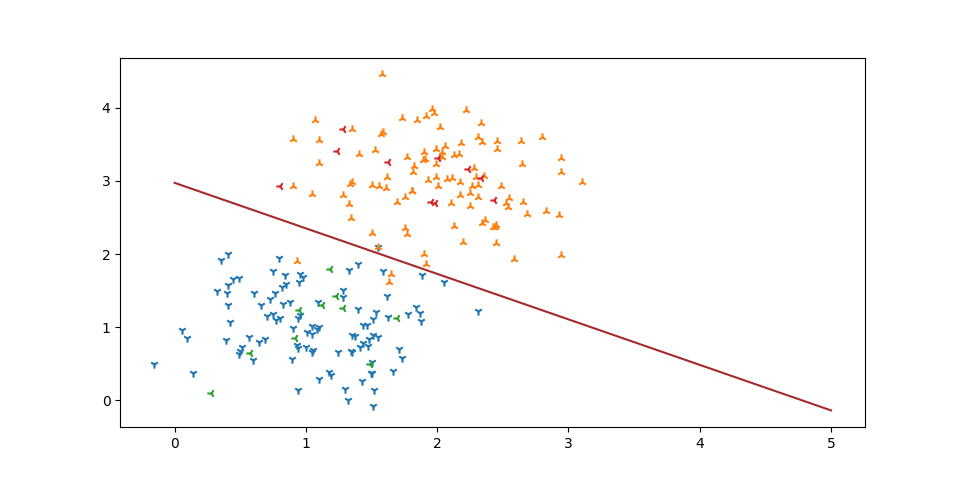
\includegraphics[height=8cm]{Figure_1.png}
        \caption{正类和负类样本中心为$(1,1)$和$(2,3)$,对应蓝色点和橙色点。测试点绿色正类,红色为负类。}
    \end{minipage}
 \end{figure}
 由程序运行结果得到验证集准确率
 \begin{python}
    acc is 1.0
 \end{python}
 \subsection*{\Large 附加题一}
 {\large\textbf{调整学习率参数以及迭代步数,画出超平面观察更新中的超平面是如何变化的。}}


 在实际验证过程中,达到要求需要的迭代次数超过2000次。这里我们给出每200次次迭代的超平面集。
 \begin{figure}[H]
    \centering
    \begin{minipage}[t]{1.0\linewidth}
        \centering
        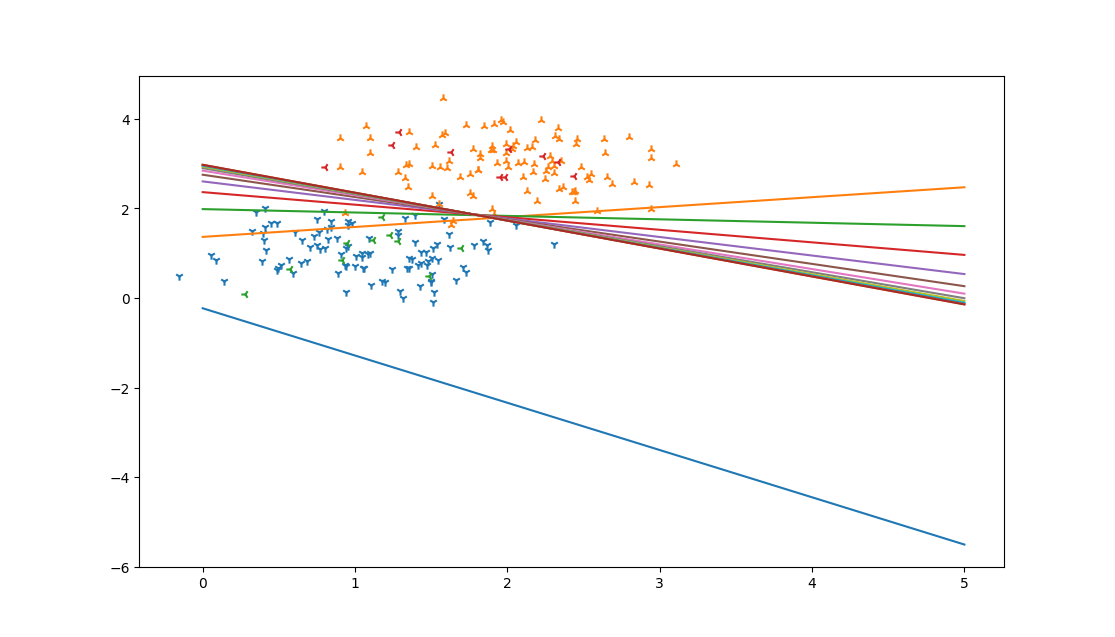
\includegraphics[height=8cm]{Figure_2.png}
        \caption{蓝色的超平面是随机初始化参数的超平面,其他的则是每200次迭代的超平面}
    \end{minipage}
 \end{figure}


 从图像中可以看到,随着迭代次数的增加,超平面参数的调整趋于稳定,最终收敛到一个最佳超平面上。
 \subsection*{\Large 附加题二}
 {\large\textbf{比较梯度下降法和课本中更新算法的结果}}\\


 除了梯度下降法更新参数,我们也可以通过最小化
 $$min_{\omega,b}-\sum_{i = 1}^{n}  (\omega^T\overrightarrow{x_i}+b )y_i$$
 来更新模型参数,这里我们简单给出模型学习的过程:对于训练样本中的任意一个样本$x_i$,如果$(\omega^T\overrightarrow{x_i}+b )y_i\leq 0$
 那么就更新参数$$\omega_{k+1}=\omega_k+\eta y_ix_i$$
 $$b_{k+1}=b_k+\eta y_i$$
 然后再次计算$(\omega^T\overrightarrow{x_i}+b )y_i$,如果对于任意的$x_i$都有这个值大于$0$,那么说明所有的样本都被正确分类,结束学习。

 \begin{python}
def objective_function(omega_and_bias:np.ndarray,data_x:np.ndarray,data_y:np.ndarray):#data is a single sample
    return data_y*(omega_and_bias[0:-1]@data_x.T+omega_and_bias[-1])
def optmize(omega_and_bias:np.ndarray,data_x:np.ndarray,data_y:np.ndarray):
    step=1e-5
    iternum=0
    while iternum<10000:
        t:np.ndarray=[]
        for i in range(0,len(data_x)):
            if objective_function(omega_and_bias,data_x[i],data_y[i])<=0 or True:
                update=np.concatenate((step*data_y[i]*data_x[i],np.asarray([step*data_y[i]])),axis=0)
                omega_and_bias+=update
            t=objective_function(omega_and_bias,data_x,data_y)
        if t.min()>0:
            break
        iternum+=1

 \end{python}
由于这个学习方法的终止条件是所有样本都被正确分类,如果我们在生成随机样本的时候,样本方差较大,个别样本无法被正确分类,那么这种算法就没法停止学习。
因此必须要设置一个迭代次数的上限,这里我们设置为$10000$次,同样的随机样本,结果图如下。
\begin{figure}[H]
    \centering
    \begin{minipage}[t]{1.0\linewidth}
        \centering
        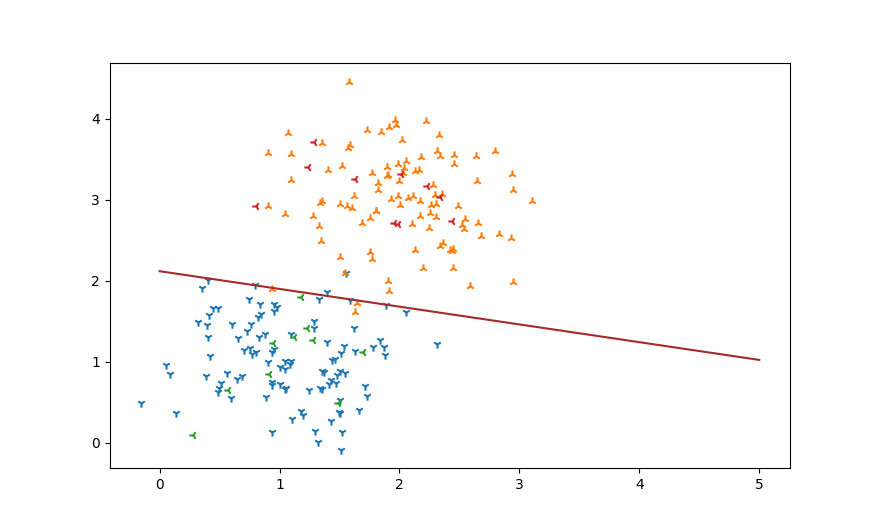
\includegraphics[height=8cm]{Figure_3.png}
        \caption{最后计算出来的超平面结果。}
    \end{minipage}
 \end{figure}
可以看到对于测试样本,这个超平面并没有全部分类正确而是有一定的误差。
如果我们缩小方差,那么这个算法就可以避免一直达不到推出条件的问题,我们重新设置$\sigma=0.2$,得到结果图
\begin{figure}[H]
    \centering
    \begin{minipage}[t]{1.0\linewidth}
        \centering
        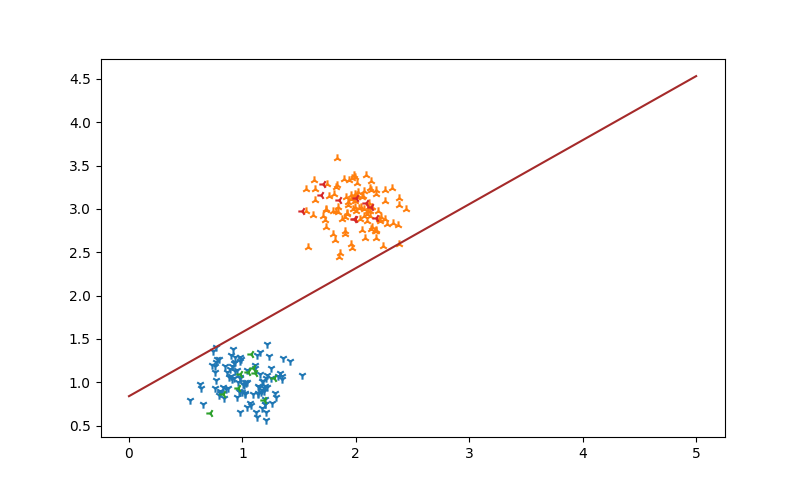
\includegraphics[height=7.5cm]{Figure_4.png}
        \caption{最后计算出来的超平面结果,可以看到这次所有的测试样本都可以被正确分类了,迭代次数为$7305$。}
    \end{minipage}
 \end{figure}


 与之对应的,如果我们采用梯度下降法,得到的结果图
\begin{figure}[H]
    \centering
    \begin{minipage}[t]{1.0\linewidth}
        \centering
        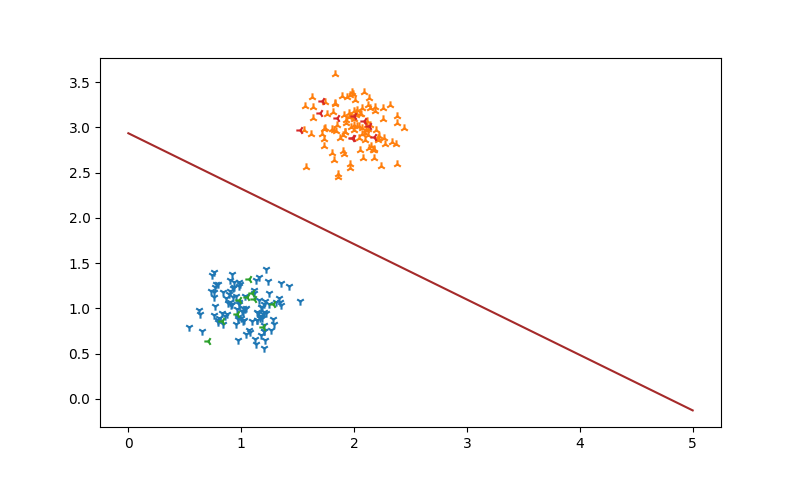
\includegraphics[height=7.5cm]{Figure_5.png}
        \caption{梯度下降法得到的结果。}
    \end{minipage}
 \end{figure}
 从结果上来看,其实梯度下降法的计算结果对于预测未知样本来说更加好,因为它保持了对两类样本都有一段距离,可以尽可能减小误差。
 这也是因为这里的算法的迭代停止条件是完全正确分类训练样本。对于所有的可接受计算结果,还存在更好的超平面,但是这里的这个算法并没有计算。


 \subsection*{\Large 附加题三}
 {\large\textbf{去掉$y_i(\omega \overrightarrow{x_i} +b)\leq 0$的条件会怎么样}}\\


 去掉这个条件的话,对于任何一个样本点,算法会无条件更新参数,可能会导致错误的训练结果。这里我们设$\sigma=0.5$,并去除条件,得到的计算结果如下
 \begin{figure}[H]
    \centering
    \begin{minipage}[t]{1.0\linewidth}
        \centering
        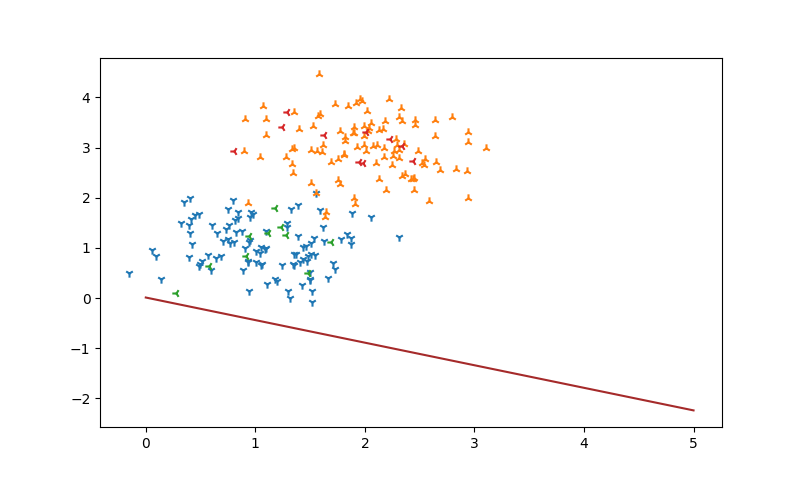
\includegraphics[height=7.5cm]{Figure_6.png}
        \caption{一个错误的计算结果。}
    \end{minipage}
 \end{figure}


 \subsection*{\Large 附加题四}
 {\large\textbf{改变样本中心使得两类样本更近或者更远,结果是怎样的}}\\

 
这里我们初始的样本中心分别是$(1,1)$和$(2,3)$ ,我们将其改为$(1,1)$和$(4,4)$,方差保持不变。利用梯度下降法,得到的结果图
\begin{figure}[H]
    \centering
    \begin{minipage}[t]{1.0\linewidth}
        \centering
        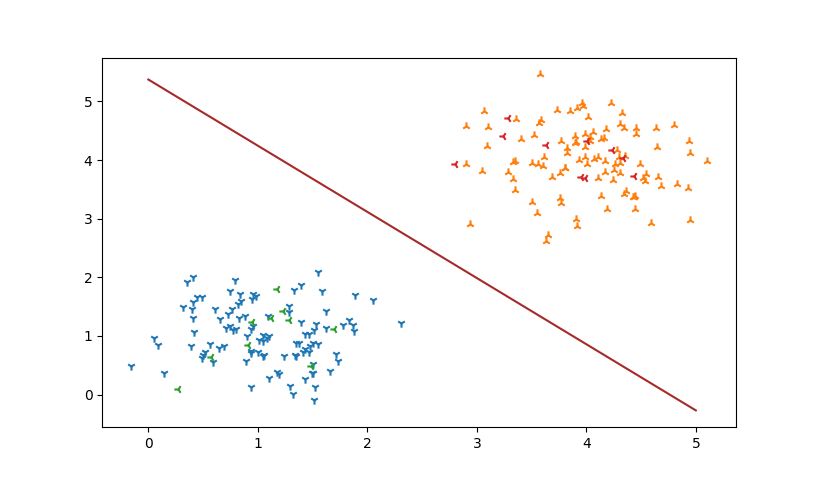
\includegraphics[height=7.5cm]{Figure_7.png}
        \caption{中心为$(1,1)$和$(4,4)$}
    \end{minipage}
 \end{figure}
 可以看出样本中心分隔越远,模型越好分类,如果我们使其中心更加靠近,设置为$(1,1)$和$(2,2)$,得到的结果图如下
 \begin{figure}[H]
    \centering
    \begin{minipage}[t]{1.0\linewidth}
        \centering
        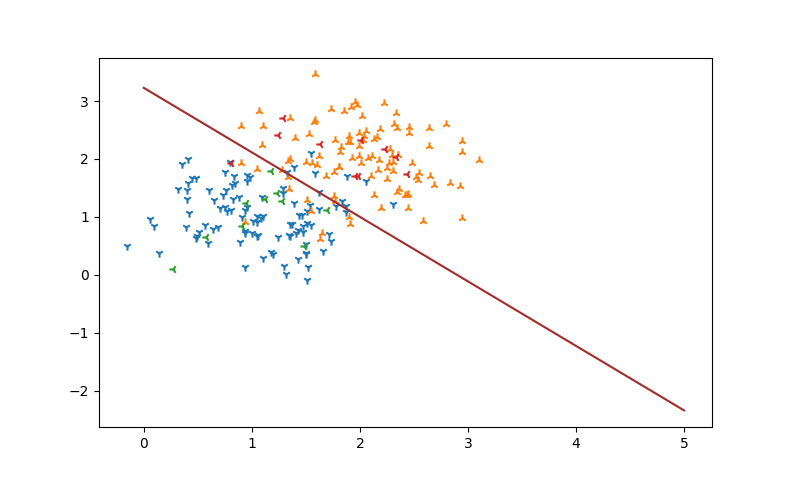
\includegraphics[height=7.5cm]{Figure_8.png}
        \caption{中心为$(1,1)$和$(2,2)$}
    \end{minipage}
 \end{figure}
这种情况下,如果方差仍然较大,那么模型不可避免会产生一定的误差,这时的两类样本也不再是完全线性的可分的。


\subsection*{\Large 附加题五}
 {\large\textbf{将数据改为高维数据如100维,生成训练数据并训练样本,报告准确率}}\\


 从理论上来说,不管样本的维数是多少,只要是线性可分的样本都可以找到一个合适的超平面来分开两类样本。但是
 在实际过程中,由于随着维数的增加,样本点之间的距离会不断变大,样本总体变得更加稀疏,所以可能会出现模型
 的分类准确率下降,甚至会出现对于同样一个方差,低维样本数据线性可分,到了高维数据就变成线性不可分了。


 实验过程中,我们首先尝试试用中心为$(1,1,\dots,1)$和中心为$(3,3,\dots,3)$的两类样本来进行模型的训练,方差
 保持为原来二维数据使用的$\sigma=0.5$,得到的准确率为
 \begin{python}
    acc is 0.6
 \end{python}
 对比之前$100\%$的准确率,显然有非常明显的下降。考虑将样本中心拉远,设置为$(-10,-10,\dots,-10)$和$(10,10,\dots,10)$,
 调整方差为$\sigma=0.1$重新训练模型,得到的准确率为
 \begin{python}
    acc is 1.0
 \end{python}
 由此可见,当维数过大的时候,方差相同的条件下高维数据更难用一个超平面分开,这就是维数灾难。
\end{document}